\cotefile{91}
\scanpage{34}

\mspage{\unsure{1|I}}

Schémas \uline{Hom} \inserted{etc.} \deleted{et calcul différentiel.}

1. Formalisme des $\mathrm{Hom}$ et $\unsure{\mathscr{V}|\mathscr{R}|\prod}_{S'/S}$

2. \deleted{Foncteurs de Greenberg.} \inserted{\unsure{Généralisation|Généralités}} Foncteurs de Serre-Lang \inserted{et} de Greenberg

3. \inserted{Existence de $W^{\unsure{\circ|\bullet}}(X)$ :} Cas affine \hfill Th.

4. \uline{Existence} \inserted{de $\underline{W}^{\circ}(X)$} : \unsure{Recollements|Résultats} \hfill Th.

5. Application aux immersions, morphismes de type fini, \hfill \rule{1.5cm}{0.35pt} affines

6. Cas des morphismes qu. projectifs \hfill Th.

% slanted
\margin{\unsure{ou plutôt|reporter} : à la fin}

\deleted{\unsure{7}}9. \deleted{\unsure{App|Ap}} Cas de $\mathscr{V}_{S'/S}$, avec $S'\unsure{-|\to}S$ étale.

\figure{\begin{tikzpicture}[x=1cm,y=1cm]\draw[->] (0,1.6) .. controls (-.55,.9) and (-.45,.1) .. (.2,-.35);\end{tikzpicture}}

\deleted{\unsure{8}}7. Cas des morphismes simples, et des morphismes étales. \hfill +Th.

[\deleted{\unsure{9}}8?] Application aux morphismes $S'\to S$ quasi-étales $[\unsure{\nu|v}(s)$ est loc. constant$]$. \hfill +Th.

[10] Compléments dans le cas de Greenberg [filtration \unsure{des|les} $W$].

% archive sheet number: 33
\scanpage{35}

\diagram{\begin{tikzcd}[ampersand replacement=\&,column sep=small]
\& X\arrow[dl,dashed,"\varphi"']\arrow[d] \& Y\arrow[dl]\\
S \& T\arrow[l,"f"] \& T\times_S T\arrow[l,bend right=15,"\mathrm{pr}_1"']\arrow[l,bend left=15,"\mathrm{pr}_2"]\arrow[ll,bend left=37,"g"]
\end{tikzcd}}

\[
f_*(X/T)=\underline{\mathrm{Hom}}_{T/S}(T/S,X/S)
\]

\[
f_*(X/T)=\underline{\mathrm{Hom}}_{S}(T,X)\times_{\underline{\mathrm{Hom}}_{\underline S}(T,T)}S
\]

\[
\underline{\mathrm{Hom}}_{T/S}(X/T,Y/T)=f_*(\underline{\mathrm{Hom}}_T(X,Y))
\]

\[
\underline{\mathrm{Hom}}_S(X,Y)=\varphi_*(X\times Y/X)
\]

\[
\underline{\mathrm{Hom}}_S(X,Y)=\underline{\mathrm{Hom}}_{S/S}(X/S,Y/S)
\]

Si $X$ est muni d'une donnée de descente : $S$, et si $f_*(X)$ existe\inserted{[et si on est \unsure{sous} les conditions d'\unsure{unicité|université|immersivité}....]}, alors l'objet descendu $X_0$ existe aussi, et on aura

\[
X_0=f_*(X)\times_{g_*(X\times_S T)}f_*(X)
\]

Contre-exemple de \uline{Nagata} : schéma algébrique simple \inserted{\unsure{absolt non-sing|abstr. non-sing}} $X$, sur un corps alg. clos $k$, avec groupe $G\simeq\mathbb{Z}/2$ opérant sans point fixe, tel que $X/G$ n'existe pas. Soit $\deleted{\unsure{K|k'}}L$ une extension de $k$ sur laquelle $G$ opère \deleted{\unsure{sans}}\inserted{\unsure{fidèlmt|fidèlem|fidèlement}} , \deleted{pt fixe} $K=L^G$, faisons opérer $G$ \uline{\unsure{diagonalemt|diagonalement}} sur $X\otimes_{\unsure{K|k}}L\,/\,L$, on a donc sur $X\otimes_k L/L$ une donnée de \uline{descente galoisienne} pour $L/K$. Je dis que \uline{le quotient n'existe pas}, i.e. \uline{la descente n'est pas possible}. En effet, \deleted{si le quotient existait, il existerait aussi par extension des scalaires \inserted{de $K$} à $\overline L$, or}

\deleted{\[
(X\otimes_kL)\otimes_K\unsure{L|\overline L}=X\otimes_k(L\otimes_KL)=X\otimes_kL
\]}

% archive sheet number: 34
\scanpage{36}

il y a \deleted{deux pts de} une trajectoire $\Gamma$ fermée de $G$ dans $X$ qui n'est pas contenue dans un ouvert affine. Cela \unsure{ns|nous} \uline{montre} que l'image inverse de cette trajectoire dans $X\otimes_k\deleted{\unsure{K}}L=\deleted{\unsure{X}}X_{K}$ est \deleted{fermée} une \deleted{trajectoire}\inserted{partie} fermée, \deleted{\unsure{sous $G$}}\inserted{qui} n'est contenue dans aucun ouvert affine. \inserted{C'est une trajectoire sous $G\times1$.}

% slanted
\margin{\uline{détailler} en donnant un \uline{lemme}}

De plus, sur cette partie, $\deleted{\unsure{G}}1\times G$ opère \unsure{trivialemt|trivialement}, donc les opérations \deleted{\unsure{du groupe}} diagonales de $G$ sont celles de $G\times1$.

\figure{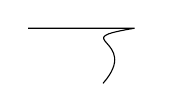
\begin{tikzpicture}[x=1cm,y=1cm]\draw (0,0)--(1.35,0) .. controls (.45,-.15) and (1.45,-.13) .. (.95,-.7);\end{tikzpicture}}

\uline{Corollaire} $\underline{\mathrm{Hom}}_{\deleted{\unsure{K}}L/K}(\deleted{\unsure{S}}\mathrm{Spec}_{\unsure{?|g}}(\deleted{\unsure{K}}L),X_{(L)})$ n'existe pas. À fortiori $\underline{\mathrm{Hom}}_K(\unsure{\mathrm{Spec}|\mathrm{Spm}}(L),X_{(L)})$ n'existe pas

On fera attention que dans cet exemple, $K$

% archive sheet number: 35
\scanpage{37}

\figure{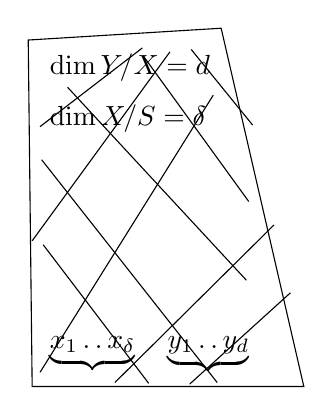
\begin{tikzpicture}[x=1cm,y=1cm]
\draw (0,0)--(-.05,4.4)--(2.4,4.55)--(3.45,0)--cycle;
\node[anchor=west] at (.1,4.05) {$\deleted{\dim Y/X=d}$};
\node[anchor=west] at (.1,3.4) {$\deleted{\dim X/S=\delta}$};
\node[anchor=west] at (.1,.4) {$\deleted{\underbrace{x_1\mathinner{\ldotp\ldotp}x_\delta}\quad\underbrace{y_1\mathinner{\ldotp\ldotp}y_d}}$};
\draw (.1,3.3)--(1.4,4.3) (0,1.85)--(1.75,4.25) (.1,.18)--(2.3,3.7) (1.05,.05)--(3.07,2.05) (2,.03)--(3.28,1.19);
\draw (.14,1.8)--(1.48,.04) (.12,2.88)--(2.35,.05) (.45,3.8)--(2.72,1.35) (1.41,4.2)--(2.75,2.35) (2.02,4.28)--(2.8,3.32);
\end{tikzpicture}}

\uline{\S1} Descente \inserted{d'objet plat} par morphismes quelconques

% slanted
\margin{intervertir ?}

\uline{\S2} Descente d'objet quelconque par morphismes plats.

\uline{\S3} Application \inserted{du \S1} aux morphismes non ramifiés

\uline{\S4} Cas particuliers élémentaires : \unsure{Espaces|Espace} $X/G$; descente galoisienne non ramifiée, le \uline{contre-exemple de Nagata}. Interprétation de la descente plate \uline{finie par quotients} \unsure{groupe|quasi} différentiel. Cas de Cartier.

% slanted
\margin{Le troisième \unsure{alinéa|ordre} du \S1 n'est pas utilisé \unsure{aux|dans les} \S\S1 à 7}

% slanted
\margin{\uline{\unsure{Considérer} descente d'un fibré} \uline{principal} ? \uline{Pas ici le} \uline{lieu}, mais \unsure{renvoyer}}

\uline{\S5} $\underline{\mathrm{Hom}}_S(X,Y)$ et $f_*(X)$ : formalisme général, cas d'existence pour $X$ fini et plat sur $S$. [Est lié à la technique de descente \deleted{\unsure{seulement}} par deux endroits a) Existence de \uline{Hom} si $X\to S$ est géom. injectif -- fini et plat -- b) Relations entre l'existence des $f_*(X)$, $\underline{\mathrm{Hom}}_S(X,Y)$, et les possibilités de descente.] Cas particuliers : $\check{V}(F)$ etc.

% slanted
\margin{propriétés diverses de permanence}

\uline{\S6} Application des schémas \uline{Hom} : la géométrie différentielle les \unsure{$P^i$ envir.|$P^i$ env.|Picard}, Greenberg d'égale caractéristique etc

% slanted
\margin{\uline{ailleurs ?} Ne vient ici que par l'utilisation dans un cas \unsure{bien banal} de l'existence de $f_*$. Pourrait venir \unsure{entièrement|aussi bien} dès le Chap \uline{IV}, mais obligerait d'y développer déjà un \unsure{bout|nº} des \uline{Hom}}

\uline{\S7} Hyper\deleted{\unsure{groupes}}\unsure{schémas|schèmes|thèses} sur $S$. Critère de représentabilité.

[y inclure aussi le critère général d'existence par théorie des modules formels]

\uline{\S8} \unsure{4|A} \deleted{\unsure{Cas particuliers}}\inserted{Théorèmes} \uline{fondamentaux d'existence}

A) Théorie formelle des modules. Extension des \unsure{sections|relations|solutions}.....

\uline{\S9} B) \deleted{\unsure{Hom}} $f_*(X)$ si $X$ est projectif sur $Y$, $Y$ plat et propre sur $S$.

\uline{\S10} C) Picard.

% slanted
\margin{ensemble ?}

[Critères de simplicité, de propreté, de platitude ?]

% archive sheet number: 36
\scanpage{38}

\uline{Proposition} Soit $f:T\unsure{-|\to}S$ un morphisme fini localement libre, et soit \deleted{\illegible{1}} $F$ un faisceau qu. coh. localement libre sur $T$, de sorte que $f_*(F)$ est un faisceau \inserted{qu. coh.} localement libre sur $S$. Alors on a un isomorphisme fonctoriel

\[
\boxed{f_*(\underline{\check V}(F))=\underline{\check V}(f_*(F))}
\]

[cet isomorphisme est compatible aux images inverses, \inserted{en particulier} localisation].

% archive sheet number: 37
\scanpage{39}

\diagram{\begin{tikzcd}[ampersand replacement=\&] X\arrow[d,"f"]\\Y=\unsure{\mathrm{Spec}|\mathrm{Spm}}(O)\end{tikzcd}}

\[
F=\widetilde M
\]

$f$ \inserted{plat et} propre, $Y$ schéma noethérien local, $F$ cohérent sur $Y$

\diagram{\begin{tikzcd}[ampersand replacement=\&,column sep=small] F'=f^*(F),\quad F'_1\subset F'\arrow[r,bend right=14] \& \text{ss faisceau cohérent.}\end{tikzcd}}

\deleted{\unsure{on}} Je dis qu'il y a un plus petit ss-faisceau cohérent $F_1$ de $F'$ t.q $f^*(F_1)\supset F'_1$

% slanted
\margin{N.B. $F$ est défini par un $O$-module $M$, les $F_i$ par des $M_i\subset M$, par \uline{définition} on pose $\unsure{\bigwedge|\bigcap}(F_i)=\widetilde{\bigcap M_i}$ [ce qui est \unsure{pas} le faisceau $\bigcap$, mais l'inf sur les faisceaux qu.coh. sur $Y$]}

Si $f_{\deleted{\unsure{*}}}^*(F_1)$ et $f^*(F_2)\supset F'_1$ alors $f_{\deleted{\unsure{*}}}^*(F_1\cap F_2)\underset{\substack{\text{platitude}\\\text{de }f}}{=}f_{\deleted{\unsure{*}}}^*(F_1)\cap f^*(F_2)\supset F'_1$, les $F_i\subset F$ tq $f^*(F_i)\supset F'_1$ \deleted{\unsure{forment}} un \deleted{filtrant} décroissant. \deleted{Il} reste à prouver que $F_1=\bigcap F_i$, alors $f^*(F_1)\supset F'_1$ i.e. l'image de $F'_1$ dans $F'/f^*(F_1)=f^*(F/F_1)$ est nulle. Remplaçant $F$ par $F/F_1$, on est ramené à prouver ceci : \uline{si} $\bigcap F_i=0$, \uline{alors} tout faisceau \deleted{\unsure{cohérent}} $F'_1$ contenu dans $\bigcap f^*(F_i)$ est nul

\margin{[est-il vrai que $\bigcap f^*(F_i)$ est nul ?]}

% slanted
\margin{Énoncé : ss les conditions envisagées, ($f$ propre, les $F_i$ décroissants dans $F$ \unsure{coh.}, $Y$ local et \unsure{noeth.}) on $\ f^*(\bigcap F_i)=\bigcap f^*(F_i)$ ?}

\deleted{$\unsure{\bigcap f^*(F_i)=0}$} ($f$ propre \deleted{\unsure{surjectif}}, les $F_i$ filtrants décr. dans $F$ cohérent, $Y$ local et noeth.). \deleted{\unsure{Comme en fait|Comme $f$} $F'_1=\unsure{\bigcap f^*}$} Comme le support de \deleted{effet $s$ une section de} $F'_1$ est fermé, il suffit de prouver qu'il ne rencontre pas $f^{-1}(y)$ ($y$ le pt fermé de $Y$) donc de prouver que si $s$ est une section de $F'_1$ sur un ouvert $U$, elle est nulle en tt $x\in f^{-1}(y)$. Or comme \deleted{\unsure{les}} $\bigcap M_i=0$, les $M_i$ tendent vers $0$ dans $M$ (?)

% slanted
\margin{\uline{Arranger les notations} !}

% archive sheet number: 38
\scanpage{40}

\diagram{\begin{tikzcd}[ampersand replacement=\&,column sep=small]
\& X\arrow[d] \& \\
S \& T\arrow[l,"f" description] \& X\times_S S'\arrow[ul]\arrow[d]\\
\deleted{\unsure{S}}S'\arrow[u] \& \& S'\times_S T=T'\arrow[ll]\arrow[ul]\arrow[u,bend right=32]\arrow[ll,shift left=3,shorten >=1.1cm,shorten <=.7cm,"\unsure{f'}"]
\end{tikzcd}}

\figure{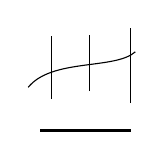
\begin{tikzpicture}[x=1cm,y=1cm]\draw[thin] (0,-.4)--(0,.4) (.48,-.3)--(.48,.42) (1,-.45)--(1,.5);\draw (-.3,-.25) .. controls (0,.12) and (.8,-.03) .. (1.06,.2);\draw[thick] (-.15,-.8)--(1,-.8);\end{tikzpicture}}

\diagram{\begin{tikzcd}[ampersand replacement=\&,column sep=small,row sep=small]
\& X_s\arrow[d] \& \\
s \& T_s\arrow[l,dash] \&\\
\& \& X'_{s'}\arrow[uul]\arrow[dl]\\
s' \& T'_{s'}\arrow[l,dash]\arrow[uu]\arrow[ur,dashed,bend right=35] \&
\end{tikzcd}}

\uline{Proposition 2} Supposons que $f_*(X/T)$ existe, et que pour tt $s\in S$, \deleted{toute}\unsure{tte|toute} multisection de $X_s/T_s$ définie sur une extension finie \inserted{$k'$} [\unsure{quelc.}] de $k(s)$, soit ``contenue'' dans un ouvert \inserted{d'un} \deleted{\unsure{affine d'un}} $U_i\otimes_k k'$ ($U_i$, famille donnée). Alors $f_*(X/T)$ est réunion des $f_{i*}(U_i/T)$ (\inserted{où} $f_i=f\vert U_i$).

\margin{dans le cas ``fini''}

[On suppose $T$ et $X$ de type fini sur $S$]

En effet, \deleted{soit} il suffit de montrer que \deleted{tout} pt \deleted{fermé} de $f_*(X/T)$ \unsure{provient} \deleted{\illegible{1}} \unsure{d'un|un des} $f_{i*}(U_i/T)$. Un tel pt fermé est défini par un corps $K$ sur un $k(s)$, et une \inserted{multi}section définie sur $K$ de $X_s$ sur $T_s$. On peut \unsure{le|la} supposer \deleted{définie sur une} $K$ fini sur $k(s)$, : à cause des hyp. de finitude \unsure{faites dans le|faites dans la} : \deleted{\unsure{les}} premier cas. Il provient \unsure{donc ...|d'un ...}

% slanted
\margin{remplace prop. 2}

\deleted{\uline{Corollaire}}\inserted{\uline{Proposition} $2^{\mathrm{bis}}$} Supposons que tte \inserted{multi}section $X_s/T_s$ définie sur une extension finie (resp. quelconque) $k'$ de $k(s)$ soit contenue dans un ouvert \deleted{\uline{affine} \unsure{pris}} \inserted{d'}une famille $U_i$. Supposons que les $f_{i*}(U_i/T)$ existent, alors il en est de $=$ de $f_*(X/T)$.

% archive sheet number: 39
\scanpage{41}

Démonstration. On \deleted{\unsure{considère|conditions}} sait que $f_*(U_{ij}/T)$ existe \unsure{aussi}, il s'envoie par imm. ouverte dans \deleted{les} $f_*(U_i)$ \uline{et} $f_*(U_j)$. Les conditions de cohérence sont \unsure{manifestemt} vérifiées, d'où un préschéma $\underline H$ sur $S$, \deleted{\unsure{on a une}} réunion d'ouverts $H_i\simeq f_*(U_i/T)$.

On déduit par \unsure{recollmt|recollement} un $T$-hom $H\times_S\deleted{\unsure{S}}T\to X$, \inserted{\deleted{\unsure{induisant|induit|universels}} $H_i\times T\to U_i$.} Je dis que ce dernier définit $T$ comme un \deleted{\unsure{Hom}} $f_*(X/T)$.

% slanted
\margin{On vérifie sans difficulté que $H_i$ est le plus gr\textsuperscript{d} ss-ouv de $H$ \deleted{\unsure{contenu}} dont l'image inverse dans $H\times_S T$ est dans l'image réciproque de $U_i$}

Soit $S'\to\deleted{\unsure{H|S}}$ \deleted{\unsure{un schéma, prouvons}} \inserted{sur $S$, il faut \unsure{savoir|prouver}} que $\mathrm{Hom}_S(S',H)\xrightarrow{\sim}\mathrm{Hom}_T(S'\times_S T,X)$.

On peut supposer $S=S'$.

\deleted{La flèche est \uline{injective}, car si on a \deleted{\unsure{une section}}\inserted{deux} $\deleted{\unsure{S\to T|S'\to S}}$, \deleted{\unsure{la s :}} sections \deleted{\unsure{$s',s''$}} $u,v:S\to H$ définissant le $=$ \deleted{application}\inserted{morphisme} $T\to X$, les images inverses $T_i$ par ce dernier \deleted{\unsure{de $U_i$|ouverts}} des $U_i$ \uline{recouvrent} $T$,}

\diagram{\begin{tikzcd}[ampersand replacement=\&,column sep=small,row sep=small]
\deleted{S}\arrow[r,dash]\arrow[d,dash] \& \deleted{H}\arrow[d,dash]\\
\deleted{\unsure{S\times T|S'}}\arrow[r] \& \deleted{\unsure{S|T}}
\end{tikzcd}}

\diagram{\begin{tikzcd}[ampersand replacement=\&,row sep=small,column sep=small]
\& X\arrow[d]\supset U_i \&\\
S \& T\arrow[l] \&\\
H\arrow[u] \& \& H\times_S T=\bigcup H_i\times_S T\arrow[ll]\arrow[ul]\arrow[uul,bend right=18]
\end{tikzcd}}

i.e. il faut prouver $\mathrm{Hom}_S(S,H)\simeq\mathrm{Hom}_T(T,X)$\unsure{.:|.|,} Soit $\varphi$ une section de $X/T$,

% archive sheet number: 40
\scanpage{42}

d'après l'hypothèse \deleted{les $\unsure{s|\varphi|f}^{-1}(U_i)$ \uline{recouvrent} $T$ ;} \deleted{pour tout} $s\in S$, il existe un $i(s)$ tel que $\varphi(T_s)\subset U_{i(s)}$ et il en résulte (préciser) que l'on peut trouver un voisinage \deleted{\unsure{ou|un}} $V_{(s)}$ de $s$ tel que $\varphi(T\mid V_{(s)})\subset U_i$. On en déduit un hom $V(s)\longrightarrow H_i$, d'où $V(s)\unsure{-|\longrightarrow} H$. Il faut montrer que ça se recolle. C'est straight-forward \unsure{\ldots}.

\uline{Théorème} On suppose $T$ fini et loc. libre sur $S$, \deleted{et $X/S$ quelconque. Pour que $\operatorname{Hom}$} On suppose de plus que \deleted{\unsure{$T/S$ soit de|$T\to S$ soit de} l'\uline{une} des deux conditions suivantes (i) $T\unsure{-|\to} S$ est géom. injectif (ii)}

\margin{$k(s)\qquad k(t)$}

Pour tout $t\in S$, tte multisection de $X_s$ sur $T_s$, définie sur une extension finie de $k(s)$, soit contenue dans un ouvert affine de $X$. Alors \deleted{$\operatorname{Hom}$} \deleted{[condition tjrs remplie si tte partie} $f_*(X/T)$ existe, et est réunion des $f_{i*}(U_i/T)$, où $U_i$ parcourt les ouverts affines de $X$.

% archive sheet number: 41
\scanpage{43}

\uline{Cor. 1} La dernière hyp. abracadabrante est vérifiée dans chacun des deux cas suivants

(i) $T/S$ est géométriquement injectif

(ii) $S=\bigcup S_i$ ($S_i$ ouverts) tels que tte \inserted{partie finie de} $X\mid S_i$ soit contenue dans un ouvert affine. [p. ex. $X$ quasiproj. sur $S$].

\uline{Cor. 2} Sous les conditions du \unsure{thm|th.}, soit $X'$ un ss-schéma fermé de $X$, \inserted{soit $f'=f\mid X'$.} Alors $f'_*(X')$ existe, et est un ss-schéma \uline{fermé} de $f_*(X)$.

% archive sheet number: 42
\scanpage{44}

\diagram{\begin{tikzcd}[ampersand replacement=\&]
\& X\arrow[d]\\
S\& T\arrow[l,"f"']
\end{tikzcd}}

$f_*(X/T)$ \qquad $T$ fini sur $S$

\diagram{\[
\begin{array}{llll}
\text{si}&X/T\ \text{est affine},&f_*(X/T)\ \text{aussi}.&\\
\text{si}&\text{---}\left\{\begin{array}{l}\text{projectif}\\\text{propre}\end{array}\right.\ast&
\left.\begin{array}{l}\text{---}\\[-.4ex]\phantom{\text{---}}\end{array}\right\}&\text{\uline{pourvu que} } f\ \text{\uline{séparable}}\ (*)\\
\text{si}&\text{quasi-projectif},&\text{---}&
\end{array}
\]}

% slanted
\margin{donner un énoncé ``général'' dans le cas où $f$ est fini \uline{étale}}

\unsure{Le calcul|Le foncteur|Notons} $f_*$ est exact à gauche, \deleted{mais pas en tout exact} \inserted{en particulier}

\[
f_*(T/T)=S,\quad f_*(X\times_T Y/T)=f_*(X/T)\times_S f_*(Y/T),\quad f_*(X\times_Z Y/T)=f_*(X/T)\times_{f_*(Z/T)}f_*(Y/T)
\]

Le foncteur $f_*$ transforme imm. ouvertes en imm. \deleted{\unsure{fermées}} \inserted{ouvertes} et \unsure{sous} une légère réserve, [\deleted{\unsure{pour que|il ne suffit}} $f_*(X/T)=\bigcup_i f_*(U_i/T)$, où les $U_i$ \inserted{affines} recouvrent $X$] imm. fermées en imm. fermées. \deleted{\unsure{(} \unsure{d'ailleurs, à réserve,|et, à réserve,}}

\margin{$*$ Se voit par descente : Si $Y/S$ est tel que $f^*(Y)/S'$ soit propre resp. projectif, alors $Y/S$ l'est [Dans le deuxième cas, on suppose $T/S$ fini et plat sur $S$ \uline{loc. noeth} \deleted{\unsure{(}}], (i) \deleted{\unsure{fau|faut}} devrait dans le cas actuel pouvoir l'exorciser, en se ramenant au projectif type, \deleted{\illegible{2}} travaillant sur $\underline{\mathbb Z}$ en définitive ; il faut prouver ceci : Si un faisceau loc. libre inversible $\underline L$ sur $X$ est $T$-ample, alors $f_*(\underline L)$ (qui est un faisceau loc. libre de rang $d$ sur $f_*(X/T)$ est tel que $\det f_*(\underline L)$ est $S$-ample \ldots}

\margin{Dans le premier cas, on utilise le lemme de Chow, en notant que si $X'\longrightarrow X$ est surjectif, alors $f_*(X')\to f_*(X)$ l'est -- \deleted{par descente}, on peut pour cela supposer $S=\operatorname{Spec}(k)$, et opérer par descente \ldots Ici il faut $S$ \deleted{\unsure{noe.}} \inserted{loc.} noeth.}

\margin{\uline{Question} Si $T/S$ est fidèl'mt plat sans plus, et $\deleted{\unsure{X}}Y/S$ est tel que $Y\times_S T/T$ soit propre, est-il vrai que $Y/S$ l'est ? -- Oui dans le cas $S$ loc. noeth, car on utilise encore le lemme de Chow.}

[N.B. cette réserve doit pouvoir être levée par la technique de descente]. De $=$, \inserted{\unsure{dans le $=$ voisin. et récipro ? réserve|dans le $=$ énoncé et récipr. ? réserve}.} $f_*$ transforme \deleted{\unsure{applicat.|affines}} morphismes affines en morphismes affines [en effet, soit $\varphi:X\unsure{-|\to}Y$ affine, \deleted{alors} on est ramené \inserted{par excision} au cas où $Y$ est affine et $X\subset Y\deleted{\unsure{\times|\otimes}}\times_T Z$ \deleted{\unsure{$Z/T$, $Z$|$Z$, $\subset$, $Z$}} $X$ ss schéma fermé, \inserted{$Z/T$ affine,} et on se ramène au cas où $X=Y\mathbin{\otimes}_T Z$ puis on traite des imm. fermées] il transforme morphismes projectifs en morphismes projectifs si $T/S$ est séparable, et en tous cas il transforme morphismes quasi-projectifs en morphismes quasi-projectifs.

[$\overline{\mathrm M}$ méthode, du moins si \inserted{si on $X_{/T}\to Y_{/T}$} $Y$ est \deleted{\unsure{noeth.}}. \deleted{\unsure{donc}} qu. proj. de type fini sur $T$ donc un faisceau coh. sur $Y$ est quotient d'un provenant de $T$ ; Il vaut mieux, et il est plus précis, de prouver encore que : un

% archive sheet number: 43
\scanpage{45}

prenant le det du faisceau descendu, on trouve à partir d'un faisceau \unsure{sur ample|très ample|rel. ample} sur $X/Y$, un faisceau ample sur $f_*(X/T)/f_*(Y/T)$ \deleted{etc}]. Kif-kif pour propre.

\uline{Proposition} Soit $g:X_{/T}\to Y_{/T}$ un morphisme, et soit $\underline L$ un faisceau inversible sur $X$ \uline{ample} \deleted{pour} (resp. très ample) pour $g$. Alors $\det f_*(\underline L)$ est un faisceau ample (resp. très ample) pour $f_*(X/T)\longrightarrow f_*(Y/T)$

Démonstration. \textcircled{2} on peut supposer $Y$ affine, \inserted{(Sous la réserve faite)} l'amplitude \deleted{de \unsure{très-amplitude|très amplitude}} étant une notion locale. $^{(1)}$ On \deleted{\unsure{voit par un|voit par ce} \unsure{que|qui} en \unsure{endroit}} \inserted{est ramené au cas ``ample''.} De plus, on est ramené à prouver ceci : Si $X=P^m_Y$, et $\underline L$ le faisceau fondamental dessus, \deleted{alors} $f_*(\underline L)/T)$ \deleted{est} définit une immersion projective fermée de $f_*(P^m_Y)$ par rapport à $f_*(Y/T)$. Mais utilisant la commutation de $f_*$ avec les produits, on est ramené au cas où $Y=T$. De plus, la question étant locale, on peut supposer $S$ affine $=\operatorname{Spec}(A)$, $T=\operatorname{Spec}(B)$, $B$ étant libre de type fini (rang $d$) sur $A$.

\margin{$f_*(\unsure{X/T|U/T|\mathrm{Ker}})\longrightarrow f_*(Y/T)$ \qquad $S\qquad T$}

% slanted
\margin{\deleted{N.B. \unsure{théorème|théor.|Résultat} s'améliore si on introduit sur $Y$ le faisceau $g_*(\underline L)$ (par hypo fini ou quasicoh.) \uline{pourvu} \uline{que} (i) les \deleted{\unsure{foncteurs}} ouverts \unsure{d'imm.|d'une} projectives marchent bien sans réserve aucune. (ii) On le prouve pour un \uline{tel} faisceau quasi-cohérent}}

On est ramené \deleted{au} à deux vérifications :

A) Détermination de la grassmannienne. et d'un faisceau ample dessus, \deleted{\unsure{id.|i.e.}} d'une immersion projective de la dite.

% archive sheet number: 44
\scanpage{46}

B) Étude de la situation suivante : On a un préschéma $G$ [la grassmannienne en question] un faisceau loc. libre de rang $d$ d'algèbres $\underline A$ sur $G$ (l'image inverse de $f_*(\underline{\mathcal O}_T)$] un faisceau loc. libre de $\underline A$ \deleted{\unsure{alg.}}-modules $\underline F$, un sous-faisceau de $\underline O_G$-\deleted{\unsure{alg.}}modules $\underline F_1$, \inserted{tel que $\underline F/\underline F_1$ soit} loc. libre de corang $kd$. On s'intéresse, pour tt préschéma $G'$ sur $G_{\unsure{T|S}}$ [\unsure{sans|sur|sens|exemple} $G\times_{\unsure{S|T}} S'$] de savoir si \deleted{$\underline F'_1\subset\underline F'$ est un \unsure{ss-module|$B$-module|ss-schéma} \unsure{mod. de}} \inserted{$\underline F'_1/\underline F'$ est loc libre de} rang $k$ \uline{sur $\underline A'$}. On veut définir un ss-schéma \deleted{fermé} $G_{\unsure{\ast|k|A}}$ de $G$ tel que la cond. néc. et suff. cherchée soit que $G'\to G$ se factorise par $G_{\ast}$.

La \deleted{condition} \inserted{question} étant \uline{locale} sur $G'$ (détermination de la représentabilité d'un foncteur !), on peut supposer : \deleted{$\underline F=\underline A^n,\ \underline F_1=$}

(i) \deleted{$\unsure{S|T}$} $G$ affine d'anneau $A$

(ii) $\underline A$ défini par une $A$-algèbre $B$ ayant une base $b_1,\ldots,b_d$

(iii) $\underline F$ défini par $B^n$, donc a une base $b_\alpha^{(i)}\left(\begin{smallmatrix}1\leq i\leq n\\1\leq\alpha\leq d\end{smallmatrix}\right)$

(iv) $\underline F_1$ a une base \deleted{$\unsure{b'_i|b_i}$} $(\unsure{c_i|c_\gamma|c_\lambda})_{1\leq i\leq(\unsure{n-k|nk})d}$, qui se complète en une base d'un supplémentaire $(d_j)_{1\leq j\leq kd}$

On va chercher \deleted{la} \inserted{une} condition néc. et suffisante

% archive sheet number: 45
